\chapter{Results}
\label{cha:results}
In the next two sections I will illustrate and discuss the results of the main two abstract components of my project: the \textit{Symptom Identifier} and the \textit{Symptom Classifier}.

\section{Evaluation of the Symptom Identifier}
In order to evaluate the Symptom Identifier, I manually classified the tokens for predictions of each sentence in four classes (just to recall, tokens for predictions are the outcome of the Symptom Identifier):
\begin{itemize}
  \item \texttt{correct} tokens. These are tokens that contain an intelligible symptom that is also present in the patient's sentence;
  \item \texttt{redundant} tokens. These tokens are correct but redundant (there is another token that has the same meaning);
  \item \texttt{non sense} tokens. These tokens are simply not intelligible;
  \item \texttt{wrong} tokens. These tokens are deceptive because they contain an intelligible symptom but they are not present in patient's sentence.
\end{itemize}

Finally, for each sentence, I noted also the number of symptoms present in the sentence but not in the tokens (\texttt{missing}).

In order to choose the best model for future evaluations, I designed a score metric that summarizes the performance of this component. Just for a matter of clarity, ``\texttt{\#C}'' means ``total number of predictions belonging to the class \texttt{C}'':
\begin{equation}
score = \texttt{\#correct} + 0 \cdot \texttt{\#redundant} - \texttt{\#non sense} - \texttt{\#wrong} - \texttt{\#missing}
\end{equation}

The reader may wonder why is a \texttt{non sense} token so penalized. The reason is that this type of token is detrimental as much as a wrong one because it leads to a random prediction. Instead, a redundant token is neutral because it probably leads to a duplicated, but correct, prediction.

Here is an overview of the obtained results:

\definecolor{green}{rgb}{0.8,0.9,0.8}
\definecolor{lightgreen}{rgb}{0.89, 0.94, 0.89}
\definecolor{red}{rgb}{1,0.89,0.89}

\begin{center}
 \begin{tabular}{| c | c | c | c |} 
 \hline
 \# of & BERT & R-NET \\ [0.5ex] 
 \hline\hline
 \rowcolor{green}
 \texttt{correct} & 423 & 427 \\ 
 \hline
 \rowcolor{lightgreen}
 \texttt{redundant} & 275 & 195 \\
 \hline
 \rowcolor{red}
 \texttt{non sense} & 122 & 247 \\
 \hline
 \rowcolor{red}
 \texttt{wrong} & 8 & 14 \\
 \hline
 \rowcolor{red}
 \texttt{missing} & 61 & 74 \\
 \hline
 \textbf{score} & \textbf{232} & \textbf{92} \\ 
 \hline
\end{tabular}
\end{center}

The results, and, in particular, the score measure, suggest that BERT is consistently better for this task. For this reason I used its outcome as input for the evaluation of the Symptom Classifier.

\section{Evaluation of the Symptom Classifier}
\subsection{Definitions and notation}

The expression ``$\texttt{real cuis}_{i}$'' refers to the list of real symptom CUIs of the i-th sentence. Analogously, the expression ``$\texttt{predicted cuis}_{i}$'' refers to the list of predicted CUIs of the i-th sentence.

The symbol ``\texttt{\#}'' in front of a list identifier indicates its length.

\subsubsection{Types of predictions}
The predictions are based on the \textit{tokens for prediction} and can be classified as:
\begin{itemize}
  \item \texttt{correct}, if the prediction is located in a subtree rooted in any of the \texttt{real cuis}. Correct predictions can be of two types:
    \begin{itemize}
      \item \textit{redundant} (\texttt{R}). When a prediction is mapped to a subtree, the subtree is marked as associated with that prediction. Then, if another prediction of the same sentence stays in that subtree, it is classified as redundant;
      \item \textit{non-redundant} (\texttt{NR}), if the prediction stays in a unmarked subtree;
    \end{itemize}
  \item \texttt{wrong}, if the prediction is not located in any of the subtrees.
\end{itemize}

Also these terms are contextual to the sentence: this means that they can be indexed as well. To give an example, $\texttt{\#correct}_{i}$ represents the number of correct predictions of the i-th sentence.

\subsection{Measures}
This component performs a slight variation of multi-class classification (a class for each symptom present in the tree). The variation stands in the ``pruning'' option (the number of candidate classes decreases) and in the fact that if the predicted CUI and the real one are different (i.e. they are different classes), the prediction could be correct (if the prediction is in the subtree of the real CUI).

Once understood the complex nature of this task, is not surprising that, apart from accuracy, there are not any standard measures used to summarize the its results. For example, precision, recall and F1 score suit only for binary classification. This led me to develop my own measures, designed exclusively for this task.

The first measure is \texttt{accuracy} and it represents the fraction of symptoms that were predicted correctly over the total number of symptoms:
\begin{equation}
\texttt{accuracy} = \frac{\sum_{i}{\texttt{\#correct}_{i}^{\texttt{NR}}}}{\sum_{i}{\texttt{\#real cuis}_{i}}}
\end{equation}

The second measure is \texttt{\% of correct predictions} and it is the fraction of the number of correct predictions (redundant and non-redundant) over the total number of predictions. This measure represents the probability, for a prediction, of being correct:
\begin{equation}
\texttt{\% of correct predictions} = \frac{\sum_{i}{\texttt{\#correct}_{i}}}{\sum_{i}{\texttt{\#predicted cuis}_{i}}}
\end{equation}

The following measure, called \texttt{medium attempts}, is computed as the total number of predictions over the total number of actual symptoms present in the sentences. It represents the medium number of attempts that the model does for each symptom a the sentence:
\begin{equation}
\texttt{medium attempts} = \frac{\sum_{i}{\texttt{\#predicted cuis}_{i}}}{\sum_{i}{\texttt{\#real cuis}_{i}}}
\end{equation}

The fourth measure represents the \texttt{missed symptoms}. Even if it is not indispensable because it is complementary to the \texttt{accuracy}, it can be useful to understand the number of missed tokens (and not its percentage):
\begin{equation}
\texttt{missed symptoms} = \sum_{i}{\texttt{\#real cuis}_{i}} - \sum_{i}{\texttt{\#correct}^{\texttt{NR}}_{i}}
\end{equation}

\subsection{Evaluation of different options}
In this subsection I will show and analyze individually every option of the Symptom Classifier. Those are: the embedding type, if using or not the \textit{Body Part Finder}, if using or not the ``pruning'' option, if using or not the \textit{filter for ``unuseful words''} and the \textit{minimum similarity} level.

\newpage
\subsubsection{Comparing different types of embeddings}

\begin{figure}[h]%[!tbp]
  \centering
  \begin{minipage}[b]{0.4\textwidth}
    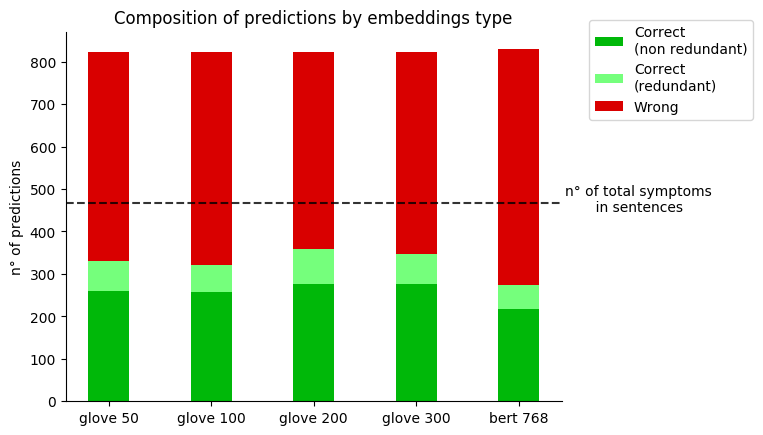
\includegraphics[width=9cm]{graphs/comparison_embeddings_type}
    \caption{Comparing the composition of the predictions across different embedding types.}
  \end{minipage}
  \hfill
  \begin{minipage}[b]{0.4\textwidth}
    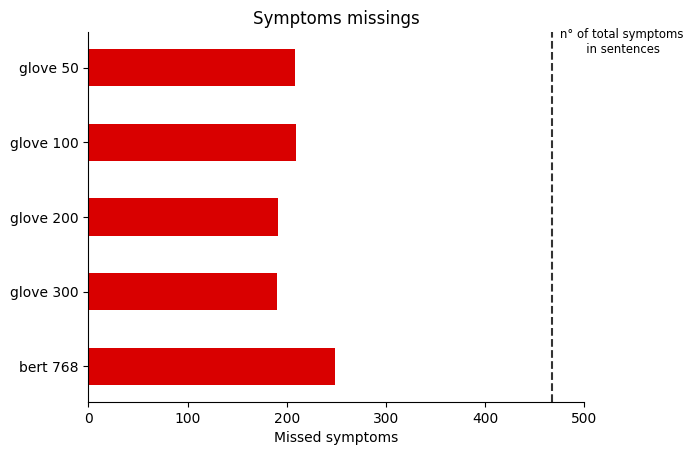
\includegraphics[width=8cm]{graphs/comparison_embeddings_type_missings}
    \caption{Comparing the \texttt{missing symptoms} across different embedding types.}
  \end{minipage}
\end{figure}

\begin{center}
 \begin{tabular}{| c | c | c | c | c |} 
 \hline
 \thead{\texttt{embedding}\\\texttt{type}} & \thead{\texttt{accuracy}} & \thead{\texttt{correct}\\\texttt{predictions}} & \thead{\texttt{medium}\\\texttt{attempts}} & \thead{\texttt{missed}\\\texttt{symptoms}} \\ [0.5ex] 
 \hline\hline
 \texttt{GloVe 50} & 55.5 \% & 40.1 \% & 1.8  & 208 \\ 
 \hline
 \texttt{GloVe 100} & 55.2 \% & 39.1 \% & 1.8 & 209 \\
 \hline
 \texttt{GloVe 200} & 59.1 \% & 43.7 \% & 1.8 & 191 \\
 \hline
 \texttt{GloVe 300} & 59.3 \% & 42.2 \% & 1.8 & 190 \\
 \hline
 \texttt{BERT emb.} & 46.7 \% & 32.9 \% & 1.8 & 249 \\
 \hline
\end{tabular}
\end{center}

%%%%%%%%%%%%%%%%%%%%%%%%%%% discuss data



%%%%%%%%%%%%%%%%%%%%%%%%%%%
\newpage
\subsubsection{Ablation test for the Body Part Finder}

\begin{figure}[h]%[!tbp]
  \centering
  \begin{minipage}[b]{0.4\textwidth}
    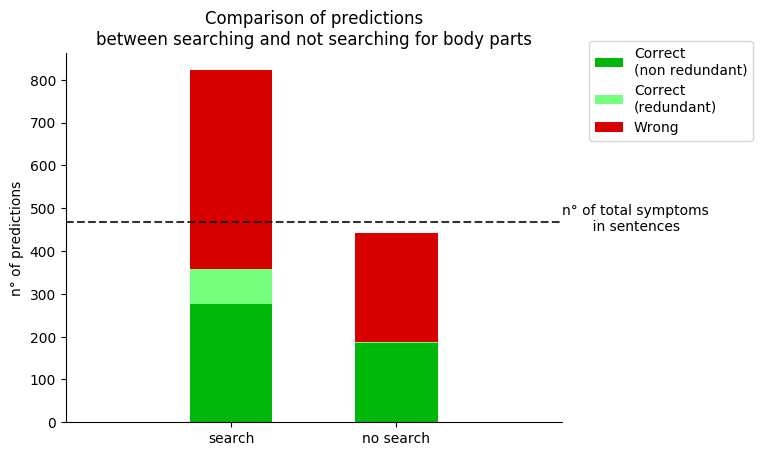
\includegraphics[width=9cm]{graphs/comparison_search_bp}
    \caption{Comparing the composition of the predictions across different embedding types.}
  \end{minipage}
  \hfill
  \begin{minipage}[b]{0.4\textwidth}
    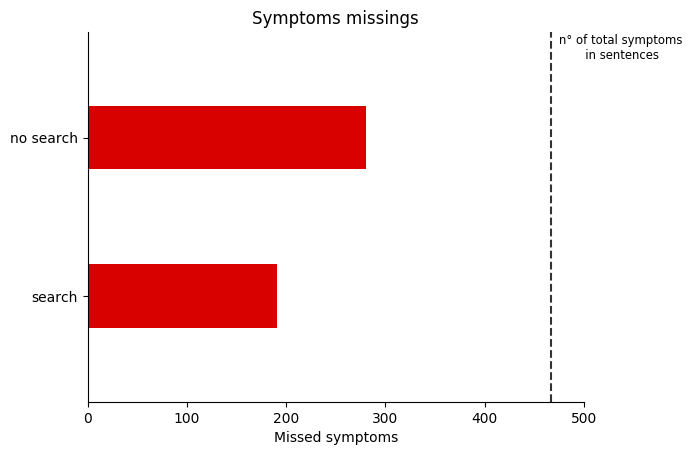
\includegraphics[width=8cm]{graphs/comparison_search_bp_missings}
    \caption{Comparing the \texttt{missing symptoms} across different embedding types.}
  \end{minipage}
\end{figure}

\begin{center}
 \begin{tabular}{| c | c | c | c | c |} 
 \hline
  & \thead{\texttt{accuracy}} & \thead{\texttt{correct}\\\texttt{predictions}} & \thead{\texttt{medium}\\\texttt{attempts}} & \thead{\texttt{missed}\\\texttt{symptoms}} \\ [0.5ex] 
 \hline\hline
 \texttt{search} & 59.1 \% & 43.7 \% & 1.8 & 191 \\
 \hline
 \texttt{no search} & 39.8 \% & 42.2 \% & 0.9 & 281 \\
 \hline
\end{tabular}
\end{center}

%%%%%%%%%%%%%%%%%%%%%%%%%%% discuss data



%%%%%%%%%%%%%%%%%%%%%%%%%%%

\newpage
\subsubsection{Ablation test for the ``pruning'' option}

\begin{figure}[h]%[!tbp]
  \centering
  \begin{minipage}[b]{0.4\textwidth}
    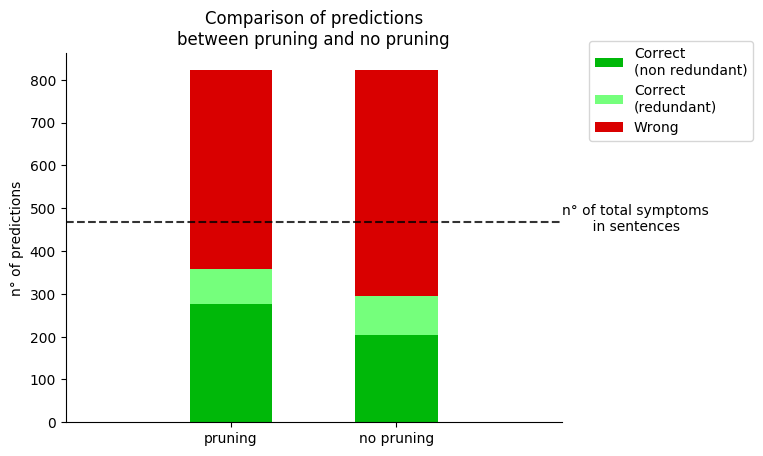
\includegraphics[width=9cm]{graphs/comparison_pruning}
    \caption{Comparing the composition of the predictions across different embedding types.}
  \end{minipage}
  \hfill
  \begin{minipage}[b]{0.4\textwidth}
    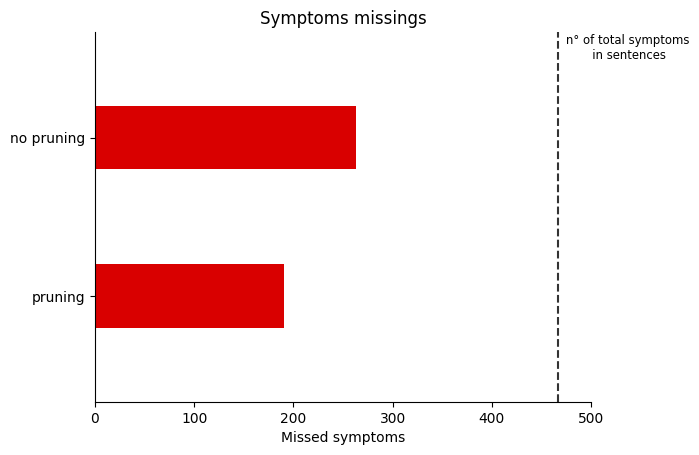
\includegraphics[width=8cm]{graphs/comparison_pruning_missings}
    \caption{Comparing the \texttt{missing symptoms} across different embedding types.}
  \end{minipage}
\end{figure}

\begin{center}
 \begin{tabular}{| c | c | c | c | c |} 
 \hline
  & \thead{\texttt{accuracy}} & \thead{\texttt{correct}\\\texttt{predictions}} & \thead{\texttt{medium}\\\texttt{attempts}} & \thead{\texttt{missed}\\\texttt{symptoms}} \\ [0.5ex] 
 \hline\hline
 \texttt{pruning} & 59.1 \% & 43.7 \% & 1.8 & 191 \\
 \hline
 \texttt{no pruning} & 43.7 \% & 36.0 \% & 1.8 & 263 \\
 \hline
\end{tabular}
\end{center}

%%%%%%%%%%%%%%%%%%%%%%%%%%% discuss data



%%%%%%%%%%%%%%%%%%%%%%%%%%%

\newpage
\subsubsection{Ablation test for the filter of ``unuseful words''}
\begin{figure}[h]%[!tbp]
  \centering
  \begin{minipage}[b]{0.4\textwidth}
    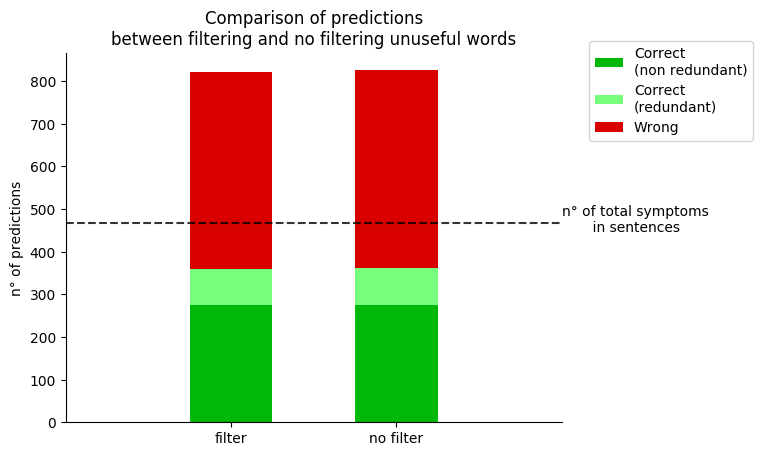
\includegraphics[width=9cm]{graphs/comparison_filtering}
    \caption{Comparing the composition of the predictions across different embedding types.}
  \end{minipage}
  \hfill
  \begin{minipage}[b]{0.4\textwidth}
    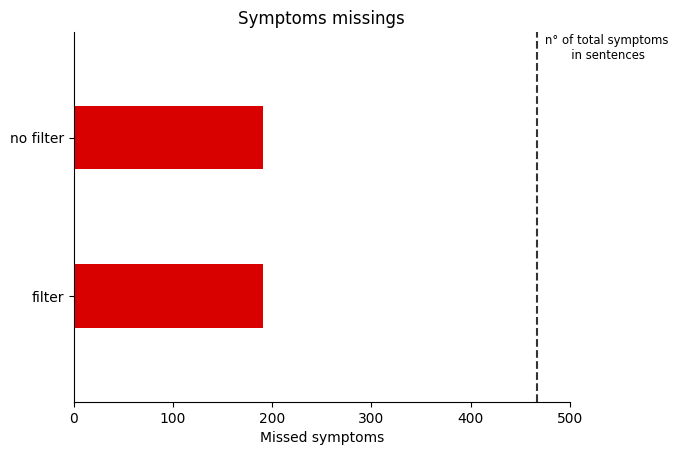
\includegraphics[width=8cm]{graphs/comparison_filtering_missings}
    \caption{Comparing the \texttt{missing symptoms} across different embedding types.}
  \end{minipage}
\end{figure}

\begin{center}
 \begin{tabular}{| c | c | c | c | c |} 
 \hline
  & \thead{\texttt{accuracy}} & \thead{\texttt{correct}\\\texttt{predictions}} & \thead{\texttt{medium}\\\texttt{attempts}} & \thead{\texttt{missed}\\\texttt{symptoms}} \\ [0.5ex] 
 \hline\hline
 \texttt{filter} & 59.1 \% & 43.7 \% & 1.8 & 191 \\
 \hline
 \texttt{no filter} & 59.1 \% & 43.9 \% & 1.8 & 191 \\
 \hline
\end{tabular}
\end{center}

%%%%%%%%%%%%%%%%%%%%%%%%%%% discuss data



%%%%%%%%%%%%%%%%%%%%%%%%%%%

\newpage
\subsubsection{Comparing different levels of \textit{minimum similarity}}
\begin{figure}[h]%[!tbp]
  \centering
  \begin{minipage}[b]{0.4\textwidth}
    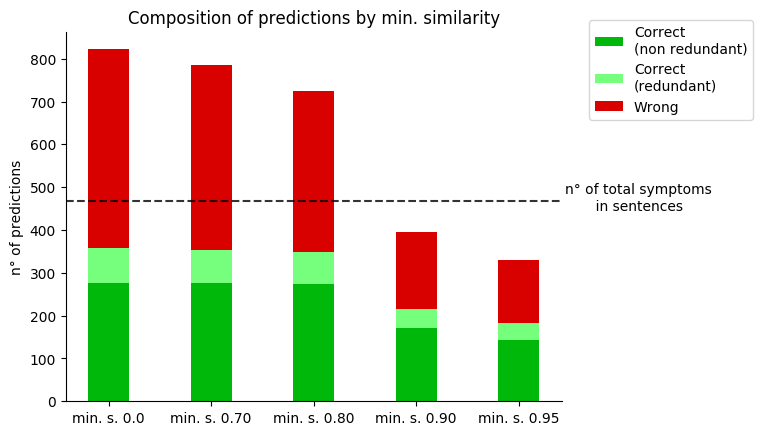
\includegraphics[width=9cm]{graphs/comparison_min_similarity}
    \caption{Comparing the composition of the predictions across different embedding types.}
  \end{minipage}
  \hfill
  \begin{minipage}[b]{0.4\textwidth}
    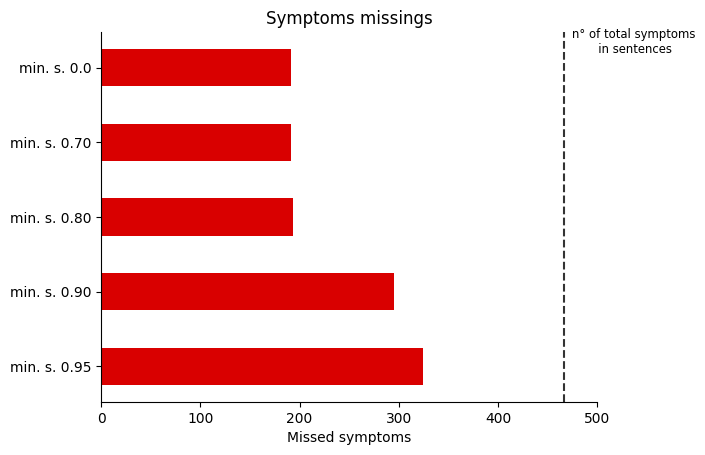
\includegraphics[width=8cm]{graphs/comparison_min_similarity_missings}
    \caption{Comparing the \texttt{missing symptoms} across different embedding types.}
  \end{minipage}
\end{figure}

\begin{center}
 \begin{tabular}{| c | c | c | c | c |} 
 \hline
  \thead{\texttt{minimum}\\\texttt{similarity}} & \thead{\texttt{accuracy}} & \thead{\texttt{correct}\\\texttt{predictions}} & \thead{\texttt{medium}\\\texttt{attempts}} & \thead{\texttt{missed}\\\texttt{symptoms}} \\ [0.5ex] 
 \hline\hline
 \texttt{0.00} & 59.1 \% & 43.7 \% & 1.8 & 191 \\ 
 \hline
 \texttt{0.70} & 59.1 \% & 45.1 \% & 1.7 & 191 \\
 \hline
 \texttt{0.80} & 58.7 \% & 48.0 \% & 1.5 & 193 \\
 \hline
 \texttt{0.90} & 36.8 \% & 54.7 \% & 0.8 & 295 \\
 \hline
 \texttt{0.95} & 30.6 \% & 55.3 \% & 0.7 & 324 \\
 \hline
\end{tabular}
\end{center}

%%%%%%%%%%%%%%%%%%%%%%%%%%% discuss data



%%%%%%%%%%%%%%%%%%%%%%%%%%%
